\section{Graphical User Interface}
The first task in testing the GUI's visualiser component with regards to it scalability, was to naturally reverse-engineer the database schema. Once this was completed, simple data was generated and run to test the performance and output of the visualiser with respect to the database requirements that are required by this project. 

Before connecting any of the interface to different parts of cluster, simple data had to be generated and visualised. The database used for this testing process was Xampp which runs a local Apache server. The graphical user interface developed using PHP by the creators of xampp also allowed for easier testing and verification of the database structure, giving a simple and efficient manner in which to check certain table entries against the expected values.

Connecting the visualiser to the local database server, proved to be a rather simple task. The dialog box shown in Figure \ref{fig:mysql}, allows simple routing of the GUI to different databases. 

\begin{figure}[htbp]%
\centering
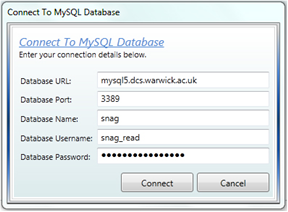
\includegraphics[width=0.5\columnwidth]{./img/mysql}%
\caption{SNAT Database Dialog Box}%
\label{fig:mysql}%
\end{figure}

However, for simplicity, the code regarding the default values was changed such that the following values were substituted in so that the database would connect straight to the Xampp server and different databases depending on what data we were testing. While not a significant step in testing, this proved to be a very useful step as it lead to increased efficiency in the testing process.

\begin{table}[htbp]%
\centering
\begin{tabular}{l|l}
Setting & Value \\
\hline
dbURL.Text & ``localhost'' \\
dbPort.Text & ``3306'' \\
dbName.Text & ``resultstesting'' \\
dbUsername.Text & ``root'' \\
dbPassword.Password & `` '' \\
\end{tabular}
%\caption{}
%\label{}
\end{table}

The next step after testing simple graphs were to test various size graphs to determine the absolute limit of the visualiser and thus determining the suitability of the visualiser. The various databases used are shown in Figure \ref{fig:phpmyadmin}

\begin{figure}[htbp]%
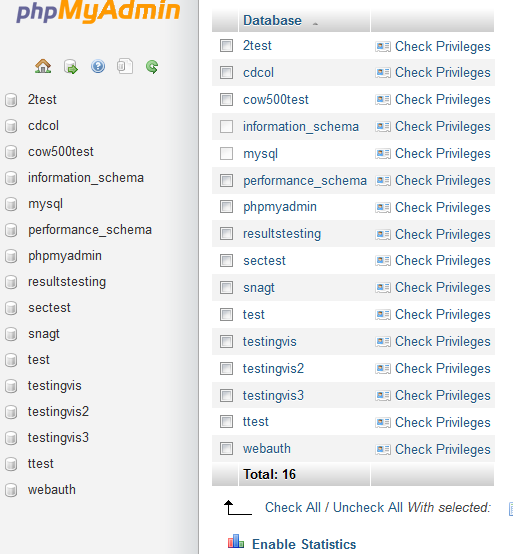
\includegraphics[width=\columnwidth]{./img/phpmyadmin}%
\caption{Databases used testing of visualisation component of GUI}%
\label{fig:phpmyadmin}%
\end{figure}

As Xampp php upload only supports up to a maximum of 8,192KiB, it was necessary to begin compressing the database into zip files, such that they could be uploaded to the local server. However, when this process proved to be limiting with respect to pushing the limits of the visualiser, alteration to the configuration of xampp was needed. 

The the values of upload\_max\_filesize, memory\_limit and post\_max\_size in the php.ini configuration file were altered so that the memory limit now usable would become 3/4 of the available RAM on the system. The laptop on which the visualiser was tested and developed on sports 4GB of RAM, which therefore should be enough to test the visualiser's performance in terms of scalability. 

The interface was set up in the following manner:
\begin{enumerate}
	\item The interface was set up into visual studio complete with standard
unedited code. The essential reasons being:
	
	\begin{enumerate}
		\item It was necessary to prevent errors that were created in the SOAP inclusion in the existing code
		
		\item It allowed for complete control of the visualisation environment
		
		\item Ensured that any errors were local
	\end{enumerate}
	
	\item The database management system used to connect the visualiser and the database would be xampp as the local system would rule out errors in connection such as potential corrupt data leading to false assumptions
	
	\item The interface was to only visualise data and perform no other action other than acquiring the dataset and visualising it. As such algorithms chosen were ``none'' and the dataset type, Full cluster node.
\end{enumerate}

The result of this rigorous testing saw no real problems with the visualiser until the database shown in Figure \ref{fig:2test} was selected. 

\begin{figure}[htbp]%
\centering
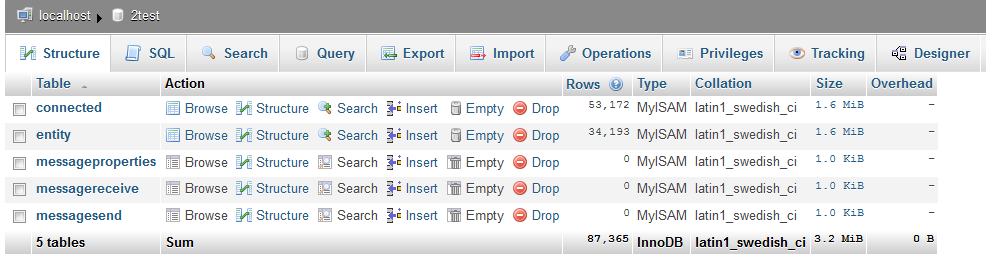
\includegraphics[width=0.5\columnwidth]{./img/2test}%
\caption{Database ``2test'' which identified 
the visualisation problems with the GUI
}%
\label{fig:2test}%
\end{figure}

As we can see from image above, the database ``2test'' was given a sample slot of data from the gathered twitter data that was currently being harvested at the time. This database was created after the completion of the reverse-engineering of the database schema and testing of correctness of the schema confirmed. The specification of the database ``2test'' is shown in Table \ref{tab:2test}:

\begin{table}%
\centering
\begin{tabular}{|l|l|}
\hline
Data & \# or Present \\
\hline
Nodes	34193
Edges	53172
Message properties & Empty (no messages) \\
Message Receive	Empty &(no messages) \\
Message Send	Empty & (no messages) \\
\hline
\end{tabular}
\caption{Database ``2test'' specification}
\label{tab:2test}
\end{table}

When this dataset was run, which was in fact a small fraction of the twitter data already harvested to that point in time, the visualiser could not cope and in fact, the system on which it was run could not handle the graphical processing involved. The system collapsed and shut the GUI and Microsoft Visual Studio reporting errors with the display adapter. This was after a 1 hour 21 minute wait for the network view model to initialise. Given the specification shown in Figures \ref{fig:hardwarespecs1} and \ref{fig:hardwarespecs2}

\begin{figure}[htbp]%
\centering
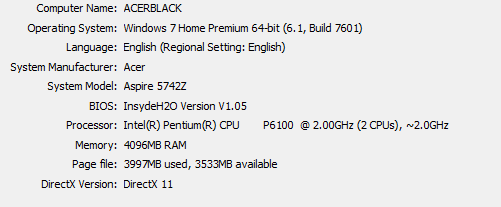
\includegraphics[width=0.5\columnwidth]{./img/hardwarespecs1}%
\caption{Specification of the system where visualisation is non-functional}%
\label{fig:hardwarespecs1}%
\end{figure}

\begin{figure}[htbp]%
\centering
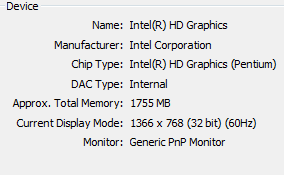
\includegraphics[width=0.5\columnwidth]{./img/hardwarespecs2}%
\caption{Graphics processing power of system in question}%
\label{fig:hardwarespecs2}%
\end{figure}

As we can see by the specification of the system, it was by no means lacking in terms of power. The conclusion that can be drawn from this experimentation is that the network view model developed by the previous group, while aesthetically pleasing, lacks scalability as a system which surpasses the system requirements specified by the previous group:

\begin{itemize}
	\item 1.6GHz or faster processor
	
	\item 1 GB (32 Bit) or 2 GB (64 Bit) RAM (Add 512 MB if running in a virtual machine)
	
	\item 3GB of available hard disk space
	
	\item	5400 RPM hard disk drive
	
	\item DirectX 9 capable video card running at 1024 x 768 or higher-resolution display
\end{itemize}

An issue identified with the visualiser however is that it is extremely
dependent on the system on which it is currently running. That is, it can only
produce large graphs with powerful systems, and the ratio of technical
specification power to graph size is currently unknown. In other-words, it is
unknown whether or not the lack of CPU power, RAM or video processing power is
the cause of the fatal crashes when trying to visualise the graphs. 

The route of testing performed, included, varying edges and node magnitudes such
that increasing values were tested, and ability of the visualiser to cope and
perform with them scrutinised. The values tested are detailed in Table
\ref{tab:lol}

\begin{table}[htbp]%
\centering
\begin{tabular}{|l|l|}
\hline
Nodes value (with no messages) & Visualisation successful  \\
\hline
100 & TRUE \\
200 & TRUE \\
500 & TRUE \\
1000 & TRUE \\
5000 & TRUE \\
34194 & 1 hour and 21 minute wait resulting in fatal system crash \\
\hline
Nodes Value (with messages) & Visualisation successful \\
100 & TRUE \\
500 & TRUE \\
1000 & 50 minute wait but TRUE \\
5000 & Unknown due to messages overloading myphp interface \\
\hline
\end{tabular}
\caption{Node magnitudes and testing of Visualisation success}
\label{tab:lol}
\end{table}

As we can see from above, the scalability of the current interface was in fact,
extremely limited. With errors and performance issues showing around the 1000
node benchmark with messages and errors developing due to a high number of nodes
and edges in a very simple graph with no edge labels in the form of messages,
one can only draw the conclusion that the scalability of the current interface
in the testing manner described is unsuitable for this project.

\subsection{Future considerations visualising large social-networks}

One of the main issues with the design and implementation of the GUI for this project, is that what is considered a small network or a large network in terms of a visualisation perspective, may in fact be considered very small networks from the notion of research only through the use of the statistical data generated. Essentially, there is a mismatch between the size of graphs that are obtainable now in terms of visualisation in comparison to the raw processing power available for just pure statistical graph analysis. Interesting propositions put forward by Rafiei et Curial \cite{rafiei} suggest that with the increase in the size of the topology and components of the graphs currently in demand by modern day researchers, a state in which sampling occurs at a progressive level within the visualisation is performed. This would lead to only small network segments becoming visualised at any given time, therefore reducing an extremely large network into smaller more easier to visualise networks.

Another consideration is that some of the most up to date visualisers for social-networks, do in fact have limitations in the size of graph they are capable of producing. For example, while the we have been able to produce graphs with cytoscape of a large size, due to the restrictions of the Java virtual machine, this again is only as powerful as the system it is run on ( and provided that the configuration files for the cytoscape software are altered to accommodate the usage of more memory for the Java virtual machine.

Further possibilities are detailed in various other papers examined such as \cite{Hu10algorithmsfor} where Hu examines the constraints involving the visualisation of large social networks as being specific problems that need to be overcome. The key enabling ingredients for generating large social network graphs include a multilevel approach, force approximations by space decomposition, and algebraic techniques for the robust solution of the stress model.

An appropriate alternative to a SOAP interface between a client visualisation application and the cluster could be the use of adaptive image manipulation in web-sites to extend the distributed nature of the project. One could design a new visualiser which is capable of processing the visualisation of the social network on a cluster. With the cluster influencing the power of the visualisation components, an image representing a sample of the graph taken and transmitted in simple quality, to the client browser. All SOAP requests can be made via the use of buttons incorporated into the site, e.g. html buttons next to visualisation window. 


% http://www.google.co.uk/url?sa=t&rct=j&q=&esrc=s&source=web&cd=1&ved=0CCwQFjAA&url=http%3A%2F%2Fciteseerx.ist.psu.edu%2Fviewdoc%2Fdownload%3Fdoi%3D10.1.1.125.9455%26rep%3Drep1%26type%3Dpdf&ei=ywyaT7HoE82r8AOXkIWZDw&usg=AFQjCNGh2l6XsX0syrUPEdMsA_2fxBp24w&sig2=GeETLDqvzZOazqJWUMI9MQ – Effectively Visualising large network through sampling- Rafiei et curial.
% http://www2.research.att.com/~yifanhu/PUB/ch16.pdf – Algorithms for Visualising Large networks by Yifan Hu